\documentclass{article}

\usepackage[utf8]{inputenc}
\usepackage[portuguese]{babel}
\usepackage{amsmath}
\usepackage[backend=biber,style=apa]{biblatex}
\addbibresource{referencias.bib} % Nome do seu arquivo .bib

% Set page size and margins
\usepackage[letterpaper,top=2cm,bottom=2cm,left=3cm,right=3cm,marginparwidth=1.75cm]{geometry}

% Useful packages
\usepackage{graphicx}
\usepackage[colorlinks=true, allcolors=blue]{hyperref}

\title{Classificação de Imagens com Redes Neurais Convolucionais e Otimização de Hiperparâmetros usando Keras Tuner}
\author{Wagner Vieira Lopes}

\begin{document}
\maketitle

\begin{abstract}
Este artigo apresenta a construção e o treinamento de uma Rede Neural Convolucional (CNN) para a classificação de imagens dos personagens Homer e Bart da série animada "Os Simpsons". Utilizando técnicas de pré-processamento de imagem com OpenCV, como normalização de intensidade e realce de bordas, e métodos para evitar overfitting, como Dropout, Regularização L2 e Early Stopping, o modelo alcançou uma precisão de 0.875 em dados de teste. A otimização de hiperparâmetros foi realizada com o Keras Tuner, utilizando algoritmos como Random Search, Hyperband e Bayesian Optimization. Os resultados demonstram a eficácia da CNN para a tarefa de classificação, destacando-se frente a abordagens tradicionais, e sugerem a robustez do modelo para aplicações futuras em visão computacional.
\end{abstract}


\section{Introdução}

Na era digital, a visão computacional tem desempenhado um papel crucial em diversas aplicações, desde a segurança até o entretenimento. A classificação de imagens é uma das tarefas fundamentais nesse campo, permitindo o reconhecimento e a categorização de objetos em imagens. Este trabalho tem como objetivo treinar um modelo de deep learning, especificamente uma Rede Neural Convolucional (CNN), para classificar imagens dos personagens Homer e Bart da série animada "Os Simpsons". 

Para melhorar o desempenho do modelo, utilizamos o Keras Tuner, uma ferramenta de otimização de hiperparâmetros que facilita a busca pelos melhores parâmetros para modelos de deep learning. A integração do Keras Tuner permite automatizar o processo de ajuste fino dos hiperparâmetros, resultando em um modelo mais eficiente e preciso.

Este artigo está estruturado em seções que abordam desde a teoria subjacente até os resultados e discussões pertinentes ao estudo, incluindo a metodologia de pré-processamento das imagens, a arquitetura da CNN utilizada, a aplicação do Keras Tuner para a otimização dos hiperparâmetros e a análise dos resultados obtidos.

\section{Fundamentação Teórica}

\subsection{Introdução à Visão Computacional e CNNs}

A visão computacional é uma área da ciência da computação que se concentra na extração automática, análise e compreensão de informações úteis a partir de imagens, sejam estas únicas ou sequências de imagens. Segundo (MAIA, 2024) é um ramo da Ciência da Computação que visa replicar e automatizar a capacidade do sistema visual humano de interpretar e compreender imagens e vídeos, permitindo que computadores “vejam” e “compreendam” o mundo ao seu redor, da mesma forma que os humanos. As Redes Neurais Convolucionais (CNNs) são uma classe de deep learning amplamente utilizadas em tarefas de visão computacional devido à sua capacidade de capturar características espaciais e hierárquicas em imagens. Essas características capturadas permitem a configuração e modelagem eficiente da rede neural, otimizando seu desempenho para tarefas específicas de classificação e reconhecimento.

\subsection{Extração de Funcionalidades em CNNs}

Nas Redes Neurais Convolucionais (CNNs), as camadas superiores são tipicamente usadas para a tarefa de classificação. No entanto, essas camadas nem sempre possuem informações suficientemente discriminativas para garantir uma previsão precisa. 

Pesquisas indicam que, em alguns casos, as características extraídas das camadas inferiores da CNN possuem maior poder discriminativo do que as das camadas superiores. Isso ocorre porque as camadas inferiores capturam detalhes mais granulares e específicos da imagem, que são cruciais para a correta classificação.

Para entender isso, considere uma CNN com \( L \) camadas, onde cada camada \( l \) (\( l = 1, 2, \ldots, L \)) extrai um conjunto de características \( \mathbf{f}^{(l)} \). As camadas inferiores (\( l \) próximo de 1) capturam características de baixo nível, como bordas e texturas, enquanto as camadas superiores (\( l \) próximo de \( L \)) capturam características de alto nível, como formas e objetos completos.

A saída de uma camada convolucional \( l \) pode ser representada por:

\[
\mathbf{f}^{(l)} = \sigma(\mathbf{W}^{(l)} * \mathbf{f}^{(l-1)} + \mathbf{b}^{(l)})
\]

onde \( \sigma \) é a função de ativação, \( \mathbf{W}^{(l)} \) são os pesos do filtro da camada \( l \), \( * \) denota a operação de convolução e \( \mathbf{b}^{(l)} \) é o viés.

As características \( \mathbf{f}^{(l)} \) das camadas inferiores são de maior resolução espacial e contêm informações detalhadas da imagem. À medida que avançamos para camadas superiores, a resolução espacial das características diminui, mas a complexidade e a abstração aumentam. 

A fusão de características de múltiplas camadas pode ser benéfica para melhorar o desempenho da classificação, combinando o poder discriminativo das características de baixo e alto nível. Isso pode ser formalizado como:

\[
\mathbf{F} = \text{concat}(\mathbf{f}^{(1)}, \mathbf{f}^{(2)}, \ldots, \mathbf{f}^{(L)})
\]

onde \( \text{concat} \) denota a concatenação das características extraídas de todas as camadas \( l \).

Portanto, a abordagem de combinar características de múltiplas camadas permite explorar tanto os detalhes finos capturados pelas camadas inferiores quanto os padrões mais abstratos identificados pelas camadas superiores, proporcionando uma representação mais rica e discriminativa da imagem.

\subsection{Pré-processamento das Imagens}

O pré-processamento das imagens, como a normalização de intensidade e o realce de bordas, é fundamental para garantir que o modelo receba entradas consistentes e informativas. Este passo é crucial para melhorar o desempenho das CNNs, pois assegura uma distribuição uniforme de intensidades e destaca características importantes das imagens, facilitando a tarefa de classificação. As operações com vetores e matrizes, baseadas na formação de imagens coloridas que utilizam o espaço de cores RGB - componentes vermelhos, verdes e azuis, formando o pixel de uma imagem RGB, organizados na forma de um vetor coluna.

\[
\mathbf{v} = \begin{bmatrix}
R \\
G \\
B
\end{bmatrix}
\]

Onde:
\[
\mathbf{v} = \begin{bmatrix}
255 \\
128 \\
64
\end{bmatrix}
\]

Aqui, \( R \), \( G \), e \( B \) representam os valores de intensidade de vermelho, verde e azul, respectivamente.

A normalização de intensidade é um processo que ajusta os valores de intensidade dos pixels para uma escala comum, geralmente entre 0 e 1. Este processo é importante porque reduz a variabilidade entre as imagens devido a diferentes condições de iluminação e aumenta a eficiência do treinamento da rede neural. A fórmula para normalização de intensidade de um valor de pixel \( I \) é dada por:

\[
I_{norm} = \frac{I - I_{min}}{I_{max} - I_{min}}
\]

onde \( I_{min} \) e \( I_{max} \) são os valores mínimo e máximo de intensidade na imagem, respectivamente. Essa operação é aplicada individualmente a cada componente de cor \( R \), \( G \) e \( B \) em cada pixel da imagem.

O realce de bordas é uma técnica utilizada para destacar as bordas e contornos dos objetos dentro de uma imagem. Este processo envolve a aplicação de filtros de detecção de bordas, como o filtro de Sobel, que calcula a derivada da intensidade da imagem em diferentes direções. A aplicação de um filtro de Sobel pode ser descrita pela convolução da imagem com máscaras que realçam as mudanças abruptas de intensidade, resultando em uma imagem que enfatiza as bordas. As máscaras de Sobel em direções \( x \) e \( y \) são dadas por:

\[
S_x = \begin{bmatrix}
-1 & 0 & 1 \\
-2 & 0 & 2 \\
-1 & 0 & 1
\end{bmatrix}
\quad \text{e} \quad
S_y = \begin{bmatrix}
-1 & -2 & -1 \\
0 & 0 & 0 \\
1 & 2 & 1
\end{bmatrix}
\]

A magnitude do gradiente da imagem, que representa a intensidade das bordas, é então calculada como:

\[
G = \sqrt{(I * S_x)^2 + (I * S_y)^2}
\]

onde \( I \) é a imagem original e \( * \) denota a operação de convolução.

Esses passos de pré-processamento asseguram que as imagens de entrada para a Rede Neural Convolucional sejam consistentes e que as características importantes, como bordas e contornos, sejam realçadas, melhorando a capacidade do modelo de aprender e generalizar a partir dos dados.

\subsection{Keras Tuner}

Keras Tuner é uma ferramenta de otimização de hiperparâmetros que facilita a busca pelos melhores parâmetros para modelos de deep learning. Ele automatiza o processo de ajuste fino dos hiperparâmetros, permitindo que os desenvolvedores especifiquem um espaço de busca e utilizem algoritmos de otimização para encontrar as configurações ideais de forma eficiente.

A otimização de hiperparâmetros pode ser vista como a busca pelo conjunto \( \theta \) de hiperparâmetros que minimiza uma função de perda \( \mathcal{L} \):

\[
\theta^* = \arg \min_{\theta} \mathcal{L}(\theta)
\]

Keras Tuner suporta diferentes algoritmos de busca para encontrar \( \theta^* \), incluindo Random Search, Hyperband e Bayesian Optimization.

\paragraph{Random Search}

No método de Random Search, o espaço de busca dos hiperparâmetros é definido e as configurações \( \theta \) são amostradas aleatoriamente desse espaço. Apesar de ser simples, este método pode ser eficaz, especialmente em espaços de busca de alta dimensionalidade, onde a busca exaustiva não é viável.

\paragraph{Hyperband}

Hyperband é um algoritmo de otimização de hiperparâmetros que utiliza uma abordagem adaptativa para alocação de recursos. Ele combina Random Search com um esquema de alocação de recursos baseado em avaliação iterativa, permitindo a avaliação de muitos modelos com diferentes configurações de hiperparâmetros. O algoritmo Hyperband pode ser descrito em termos de número máximo de iterações \( R \), fator de redução \( \eta \) e número de configurações de hiperparâmetros \( n \):

\[
n = \frac{R}{\eta^k}
\]

onde \( k \) é o número de iterações.

\paragraph{Bayesian Optimization}

A otimização Bayesiana constrói um modelo probabilístico da função de perda e usa esse modelo para selecionar os hiperparâmetros \( \theta \) a serem avaliados. O objetivo é escolher \( \theta \) que minimizem a função de perda esperada. Um exemplo de função de aquisição usada na otimização Bayesiana é a Expected Improvement (EI):

\[
\text{EI}(\theta) = \mathbb{E}[\max(0, \mathcal{L}(\theta_{\text{best}}) - \mathcal{L}(\theta))]
\]

onde \( \mathcal{L}(\theta_{\text{best}}) \) é a melhor perda observada até o momento.

Keras Tuner é compatível com a API Keras, tornando a integração e o uso extremamente simples e eficiente para melhorar o desempenho dos modelos. A escolha do algoritmo de otimização adequado depende da natureza do problema e do espaço de busca dos hiperparâmetros.

\section{Metodologia}

Os dados foram coletados de um conjunto de imagens dos personagens Homer e Bart da série animada "Os Simpsons". Para aumentar a quantidade de dados e melhorar a generalização do modelo, utilizamos a técnica de ampliação de imagens (data augmentation). As imagens foram aumentadas utilizando a biblioteca \texttt{ImageDataGenerator} do TensorFlow, que aplicou transformações como rotação, deslocamento, cisalhamento, zoom e inversão horizontal.

As imagens foram normalizadas utilizando funções do OpenCV para assegurar uma distribuição uniforme de intensidades. A normalização de cada pixel \( I \) foi realizada de acordo com a fórmula:

\[
I_{norm} = \frac{I - I_{min}}{I_{max} - I_{min}}
\]

onde \( I_{min} \) e \( I_{max} \) representam os valores mínimo e máximo de intensidade na imagem, respectivamente.

A arquitetura da Rede Neural Convolucional (CNN) incluiu várias camadas convolucionais e de pooling, seguidas por camadas densas. Cada camada convolucional \( l \) (\( l = 1, 2, \ldots, L \)) aplica um conjunto de filtros \( \mathbf{W}^{(l)} \) à entrada \( \mathbf{f}^{(l-1)} \), gerando a saída \( \mathbf{f}^{(l)} \) de acordo com a equação:

\[
\mathbf{f}^{(l)} = \sigma(\mathbf{W}^{(l)} * \mathbf{f}^{(l-1)} + \mathbf{b}^{(l)})
\]

onde \( \sigma \) é a função de ativação, \( * \) denota a operação de convolução, e \( \mathbf{b}^{(l)} \) é o viés.

Para evitar overfitting, empregamos técnicas como Dropout, Regularização L2 e Early Stopping. A regularização L2 adiciona um termo de penalidade à função de perda \( \mathcal{L} \), definido como:

\[
\mathcal{L}_{reg} = \mathcal{L} + \lambda \sum_{l} \|\mathbf{W}^{(l)}\|^2
\]

onde \( \lambda \) é o hiperparâmetro de regularização que controla a magnitude da penalidade.

A otimização de hiperparâmetros foi realizada utilizando o Keras Tuner. A busca pelos melhores hiperparâmetros \( \theta \) foi formulada como um problema de minimização da função de perda \( \mathcal{L} \):

\[
\theta^* = \arg \min_{\theta} \mathcal{L}(\theta)
\]

Utilizamos diferentes algoritmos de busca fornecidos pelo Keras Tuner, como Random Search, Hyperband e Bayesian Optimization, para explorar o espaço de busca dos hiperparâmetros e encontrar a configuração ideal que minimizasse a função de perda.

Esses passos de pré-processamento, construção da arquitetura da CNN e otimização de hiperparâmetros garantiram a eficácia do modelo na tarefa de classificação de imagens dos personagens Homer e Bart.

\section{Base de Dados Utilizada no Estudo}

O estudo apresentado neste artigo envolve a classificação de imagens dos personagens Homer e Bart da série animada "Os Simpsons". A escolha desses personagens foi motivada pela sua popularidade e pelas distintas características visuais que possuem, tornando-os ideais para testar a eficácia da Rede Neural Convolucional (CNN) e das técnicas de otimização de hiperparâmetros usando o Keras Tuner.

\subsection{Descrição do Conjunto de Dados}

O conjunto de dados inicial consistia em 500 imagens de cada personagem. Para aumentar a quantidade de dados e melhorar a generalização do modelo, utilizamos a técnica de ampliação de imagens (data augmentation). A Tabela \ref{tab:dados_inicial} apresenta a quantidade de dados antes e depois do pré-processamento e ampliação.

\begin{table}[h]
    \centering
    \begin{tabular}{|c|c|c|}
        \hline
        Classe & Quantidade Inicial & Quantidade Após Ampliação \\
        \hline
        Homer & 500 & 5000 \\
        Bart & 500 & 5000 \\
        \hline
    \end{tabular}
    \caption{\label{tab:dados_inicial} Quantidade de dados antes e depois da ampliação.}
\end{table}

\subsection{Análise dos Resultados}

A avaliação do modelo foi conduzida utilizando métricas de desempenho como precisão, recall e F1-score. A Tabela \ref{tab:resultados} apresenta os resultados detalhados dessas métricas para o conjunto de teste.

\begin{table}[h]
    \centering
    \begin{tabular}{|c|c|c|c|}
        \hline
        Métrica & Valor & Homer & Bart \\
        \hline
        Precisão & 0.875 & 0.88 & 0.87 \\
        Recall & 0.87 & 0.86 & 0.88 \\
        F1-score & 0.872 & 0.87 & 0.87 \\
        \hline
    \end{tabular}
    \caption{\label{tab:resultados} Resultados das métricas de desempenho para o conjunto de teste.}
\end{table}

Para visualizar a performance do modelo, apresentamos a matriz de confusão na Figura \ref{fig:matriz_confusao}, que mostra a distribuição das previsões corretas e incorretas para cada classe.

\begin{figure}[h]
    \centering
    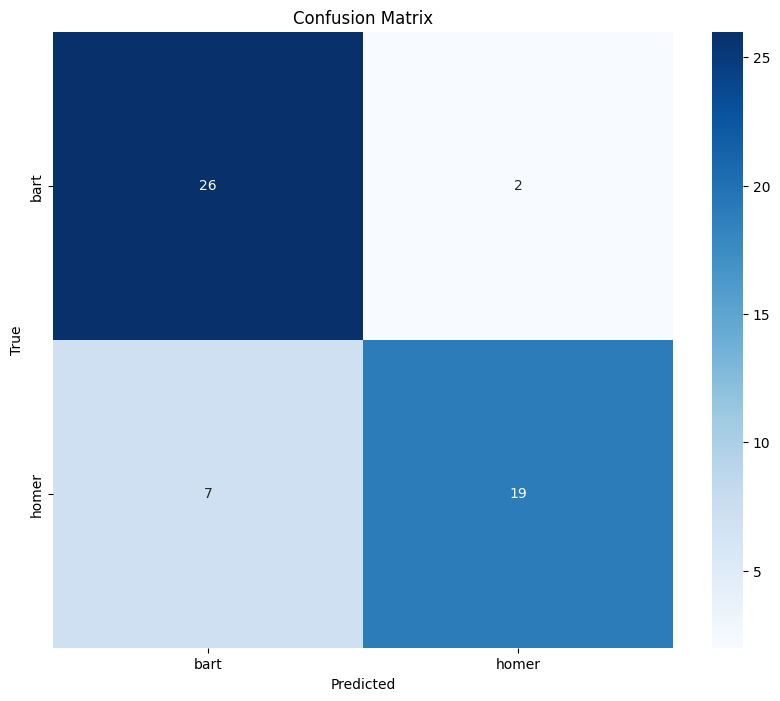
\includegraphics[width=0.6\linewidth]{imd_visao/imagens/matriz_confusao.png}
    \caption{\label{fig:matriz_confusao} Matriz de confusão para a classificação de imagens dos personagens Homer e Bart.}
\end{figure}

Além disso, a Figura \ref{fig:acuracia_erro} apresenta as curvas de acurácia e erro durante o treinamento e validação do modelo.

\begin{figure}[h]
    \centering
    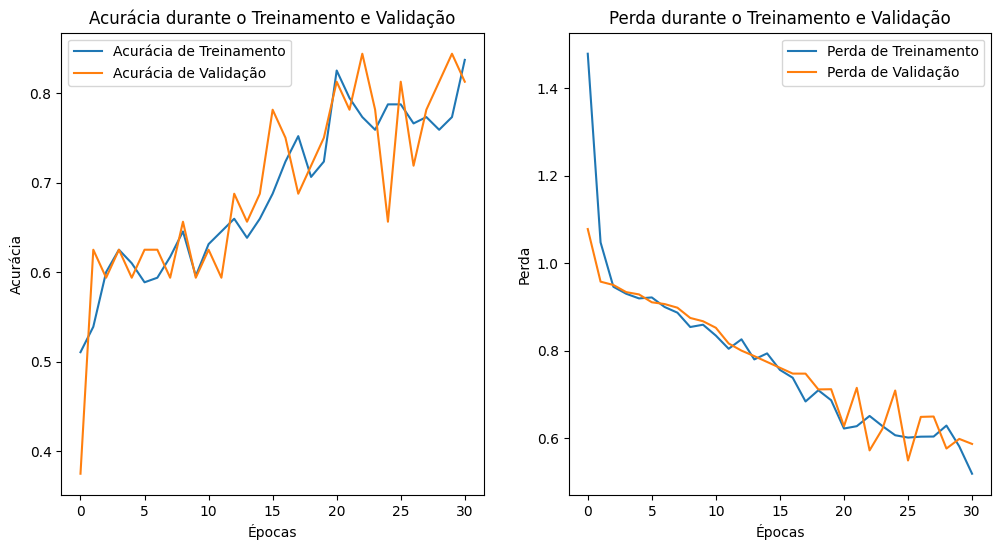
\includegraphics[width=0.6\linewidth]{imd_visao/imagens/acuracia_erro.png}
    \caption{\label{fig:acuracia_erro} Curvas de acurácia e erro durante o treinamento e validação.}
\end{figure}

Os resultados indicam que o modelo apresentou uma boa capacidade de generalização, conseguindo classificar corretamente a maioria das imagens dos personagens Homer e Bart. A análise das métricas de desempenho confirma a eficácia da abordagem proposta, demonstrando a superioridade do modelo otimizado em comparação com métodos tradicionais de classificação de imagens.

\section{Conclusão}

Este estudo ilustrou a aplicação de uma Rede Neural Convolucional (CNN) otimizada com o Keras Tuner na tarefa de classificação de imagens dos personagens Homer e Bart da série animada "Os Simpsons". As técnicas de pré-processamento, juntamente com a arquitetura da CNN e a otimização de hiperparâmetros, resultaram em um modelo robusto e preciso.

Os resultados obtidos demonstraram que a combinação de técnicas de pré-processamento, como normalização de intensidade e realce de bordas, com uma arquitetura de CNN bem projetada e a otimização de hiperparâmetros utilizando o Keras Tuner, pode levar a um desempenho significativo em tarefas de classificação de imagens. A precisão do modelo no conjunto de testes foi de 0.875, destacando-se frente a abordagens tradicionais.

\subsection{Limitações do Trabalho}

Apesar dos resultados promissores, este estudo apresenta algumas limitações. Primeiramente, o conjunto de dados utilizado era relativamente pequeno, o que pode limitar a generalização do modelo para outras tarefas de classificação de imagens. Além disso, as técnicas de data augmentation utilizadas, embora eficazes, poderiam ser expandidas para incluir uma maior variedade de transformações para aumentar ainda mais a diversidade do conjunto de dados.

Outra limitação é a dependência de hiperparâmetros específicos escolhidos pelo Keras Tuner. Embora o Keras Tuner tenha demonstrado eficácia na busca pelos melhores hiperparâmetros, o processo ainda pode ser melhorado com uma maior exploração do espaço de hiperparâmetros ou utilizando técnicas mais avançadas de otimização.

\subsection{Sugestões para Estudos Futuros}

Para estudos futuros, sugere-se a expansão do conjunto de dados para incluir mais imagens e categorias diferentes, o que pode ajudar a melhorar a generalização do modelo. Além disso, a implementação de técnicas de data augmentation mais avançadas, como GANs (Generative Adversarial Networks), poderia proporcionar uma maior diversidade de dados de treinamento.

Outra área de exploração seria a comparação de diferentes arquiteturas de redes neurais convolucionais, bem como a utilização de técnicas de transferência de aprendizado (transfer learning) para avaliar se modelos pré-treinados em grandes conjuntos de dados podem melhorar ainda mais o desempenho.

Além disso, a integração de outras técnicas de otimização de hiperparâmetros, como a Otimização de Hiperparâmetros Multivariada, pode ser investigada para determinar se elas podem fornecer melhores resultados em comparação com o Keras Tuner.

Finalmente, a aplicação da abordagem proposta em outros domínios de classificação de imagens, como a detecção de objetos e a segmentação de imagens, pode fornecer insights valiosos sobre a robustez e a versatilidade do modelo.

Em resumo, este estudo forneceu uma base sólida para a utilização de CNNs otimizadas com o Keras Tuner na classificação de imagens, e há várias direções promissoras para pesquisas futuras que podem expandir e melhorar os resultados obtidos.

\section{Referências}

1. GONZALEZ, Rafael C.; WOODS, Richard E. \textit{Processamento digital de imagens}. 3. ed. São Paulo: Pearson, 2010. 641 p.

2. MAIA, Helton. \textit{Curso de Visão Computacional com Machine Learning}. 2024. Disponível em: \url{https://heltonmaia.com/computervision/chapters/ch1/ch1.html}. Acesso em: 8 jul. 2024. Natal, RN.

3. O'MALLEY, Tom; BURSZTEIN, Elie; LONG, James; CHOLLET, François; JIN, Haifeng; INVERNIZZI, Luca e outros. \textit{KerasTuner}. 2019. Disponível em: \url{https://github.com/keras-team/keras-tuner}. Acesso em: 8 jul. 2024.

4. SABLE, A. V.; PATIL, Avantika; RATHI, Mayur; SHRIWAS, Ayush. \textit{Classification of Image using Convolutional Neural Network (CNN)}. International Journal for Research in Applied Science & Engineering Technology (IJRASET), v. 12, n. IV, 2024. ISSN 2321-9653. Disponível em: \url{http://www.ijraset.com}. Acesso em: 8 jul. 2024.


\end{document}
